\newlength{\bibsep}
\documentclass[nonatbib,5p,a4paper]{elsarticle}  % 5p for two columns, 1p for 1 column (this is specific for the elsearticle)
\usepackage[english,norsk,nynorsk]{babel}        % Language
\usepackage[DatePublished]{Code/NTNU-lab}        % remove [DatePublished] to remove dates
\usepackage{csquotes}                            % Must be loaded when babel is loaded to avoid error.
% Use this file to write code that you do not want in the .sty file, but has to be in the preamble (before \begin{document}).
% Writing in this file in stead of in the preamble will keep the main file more organised and tidy.


%                       Nomenclatures
%_______________________________________________________________
\usepackage[intoc]{nomencl}
\makenomenclature

\renewcommand{\nomname}{%
% Title
%----------------
List of Symbols
%----------------
}
\renewcommand{\nompreamble}{%
% Description
%----------------
The next list describes several symbols that will be later used within the body of the document
%----------------
}
% This code creates the groups
\renewcommand\nomgroup[1]{%
  \item[\bfseries
  \ifstrequal{#1}{A}{Physics constants}{%
  \ifstrequal{#1}{B}{Mathematical constants}{%
  \ifstrequal{#1}{C}{Other symbols}{}}}%
]}
% This will add the units
\newcommand{\nomunit}[1]{%
\renewcommand{\nomentryend}{\\#1}}
%................................................................

                            % Write all preamble code in this file to keep it organised and tidy.

%\addbibresource{Bibliography/Sources.bib}        % Selects the Bibliography file.


\begin{document}
\selectlanguage{english}                         % Sets the language of the document.

%%%%%%%%%%%%%%%%%%%%%%%%%%%%%%%%%%%%%%%%

\begin{frontmatter}
%
% Title:
%------------------------------------
\title{%
NTNU Laboratory Report Template\\
\small For Physics Reports  % A good idea is to have the subject code and name as subtitle
}
%
% Authors:
%------------------------------------
% List an author with name ' Firstname Middlename Lastname ' like this:
% F. M. Lastname
\author[NTNUphysics]{O. Nordmann} 
\author[NTNUphysics]{K. Nordmann}
\address[NTNUphysics]{Institutt for fysikk, Norges Teknisk-Naturvitenskaplege Universitet, N-7491 Trondheim, Norway.}
%
% Date:
%------------------------------------
%
\newdate{dateName}{23}{05}{2022} % edit the date here, ' dateName ' has to match on these two lines.
\renewcommand*{\today}{\MonthYearDateFormat\displaydate{dateName}} 
% Options for displaying date: \MonthYearDateFormat,  \DayMonthYearDateFormat or \YearDateFormat
%
% Abstract:
%------------------------------------
\NameOfAbstract{Abstract} % Change abstract title here. If you write in Norwegian, write 'Sammendrag' (nb) or 'Samandrag' (nn)
\begin{abstract}
% Delete the text and write your abstract here:
%------------------------------------

The abstract should be \textit{very} brief, two or three sentences may be enough. It must answer the following questions, however:
1. What did you do (What did you measure)?
2. How did you do it (which method)?
3. What did you discover (what was the results of the experiment)?
Results in form of numbers should be accompanied by an error: $R=\SI{3,05(2)e-6}{kg/s^{2}}$

\end{abstract}
%
\end{frontmatter}
%
%
% Table of contents:
%------------------------------------
% If the report is very long for some reason (over 4 or 5 pages), use a table of contents.
% Uncomment everything below the line ---- to get table of contents (ctrl + /) (the / on numberpad):
%-------------
%
% \ 
% \vspace{1cm}

% \begin{minipage}{\textwidth}
%     \tableofcontents
% \end{minipage}
% \clearpage
%% Prints a list of symbols. You can create/ change the categories in the preamble.tex file. 
% Learn more about nomenclature: https://www.overleaf.com/learn/latex/Nomenclatures
%
% Delete/change the text and write your Nomenclature here:
%------------------------------------

\nomenclature[A, 02]{\(c\)}{\href{https://physics.nist.gov/cgi-bin/cuu/Value?c}
{Speed of light in a vacuum}
\nomunit{\SI{299792458}{\meter\per\second}}}
\nomenclature[A, 03]{\(h\)}{\href{https://physics.nist.gov/cgi-bin/cuu/Value?h}
{Planck constant}
\nomunit{\SI[group-digits=false]{6.62607015e-34}{\joule\per\hertz}}}
\nomenclature[A, 01]{\(G\)}{\href{https://physics.nist.gov/cgi-bin/cuu/Value?bg}
{Gravitational constant} 
\nomunit{\SI[group-digits=false]{6.67430e-11}{\meter\cubed\per\kilogram\per\second\squared}}}
\nomenclature[B, 03]{\(\mathbb{R}\)}{Real numbers}
\nomenclature[B, 02]{\(\pi\)}{Pi}
\nomenclature[B, 01]{\(e\)}{Euler's constant}
\nomenclature[C]{\(V\)}{Constant volume}
\nomenclature[C]{\(\rho\)}{Friction index}

% Print statement:
%--------------------
\printnomenclature                 % List of symbols, can be useful
\section{Introduction}
% Delete the text and write your Introduction here:
%------------------------------------



In the feild of Machine learning there are several methods which can be used to solve the same problem. For example trying to find the local minima using eveolutionary algorithms or supervised learning in the form of back propagation. Both come with advantages and disadvantages depending on if we are after precision or just want to find the local minima fast, but also depending on the nature of our problem.

More specificaly intresssting is the comparison of the performance of Genetic Algorithms (GA) and Reinforcement Learning (RL) techniques in the context of a game environment. On one hand reinforcment learning the agent engages dynamic and evolving enviroment by taking actions that affect it in order to acomplish a specific job. On the other hand we have evolutionary algorithms which employ evolutionary princibles for automated and concurrent problem-solving by drawing inspiration from populations of interacting organisms. Despite their apparent dissimilarities, RL and GA both tackle the same fundamental issue: optimizing a function. This entails maximizing an agent's reward in RL and the fitness function in evolutionary algorithms, respectively, particularly in environments where the parameters may be unknown \cite{drugan2019reinforcement}. 

The aim of this paper is to compare Reinforcement learning and Genetic Algorthms by having them both balance a cartpole in 500 moves. 
The cart-pole balancing is a problem in non linear dynamcics where an inverted pendulum is balancing in a cart. The aim or final goal of both RL and GA are to keep it the system balanced until they run out of moves. the enviroment will be described in more detail nder the enviroment part.  
\begin{figure}[H]
    \centering
    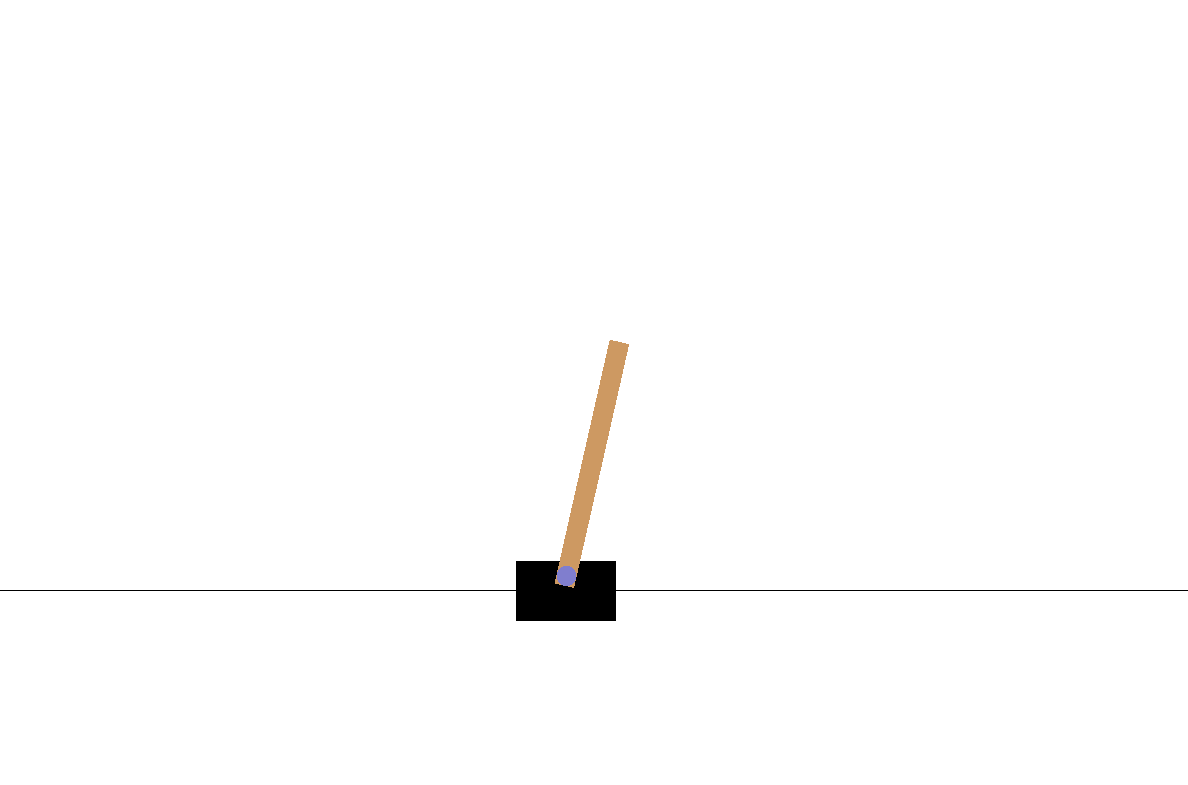
\includegraphics [scale = 0.18]{Images/cartpole.png}
    \caption{the cartpole in 2D graphics}
    \label{figPOLE}
\end{figure}
Previous work in the comparison of GA versus RL include \cite{drugan2019reinforcement} which focuses on a comperhensive overview of recent trends in the feild rather than comparisons of subclasses of algorithms or particular aspects of RL and GA. There a re also several works which focus on combining these two methods for machine learning by either using GA to train RL or vice versa such as \cite{eiben2007reinforcement} where the authurs try to use Reinforcement learnign to tune the parameters of GA. The opposite combination of training RL using GA has also been explored \cite{khadka2018evolutionary}.




%% Place large figures that span the whole width of the page in here to easily move them around in the file
% and to avoid getting figures displayed after references and appendix. 
%
% Use {figure*} for a figure that will span both columns. 
% Below is an example of a figure with 6 sub-figures.
\begin{figure*}
%
        \subfigure[Contour plot number 1]{%
            \label{fig:Contour_1}
            \includegraphics[width=0.3\textwidth]{Images/Fig:Countour-plot/1-contour.pdf}
        }%
        \hspace{1em}
        \subfigure[Contour plot number 2]{%
            \label{fig:Contour_2}
            \includegraphics[width=0.3\textwidth]{Images/Fig:Countour-plot/2-contour.pdf}
        }%
        \hspace{1em}
        \subfigure[Contour plot number 3]{%
           \label{fig:Contour_3}
           \includegraphics[width=0.3\textwidth]{Images/Fig:Countour-plot/3-contour.pdf}
        }\\ %  ------- End of the first row ----------------------%
        \subfigure[Contour plot number 4]{%
            \label{fig:Contour_4}
            \includegraphics[width=0.3\textwidth]{Images/Fig:Countour-plot/4-contour.pdf}
        }%
        \hspace{1em}
        \subfigure[Contour plot number 5]{%
            \label{fig:Contour_5}
            \includegraphics[width=0.3\textwidth]{Images/Fig:Countour-plot/5-contour.pdf}
        }%
        \hspace{1em}
        \subfigure[Contour plot number 6]{%
            \label{fig:Contour_6}
            \includegraphics[width=0.3\textwidth]{Images/Fig:Countour-plot/6-contour.pdf}
        }%
%
    \caption{%
        Contour plots for different potentials $V_0(x)$, along the line $y=1$
     }%
   \label{fig:Countour-plot}
\end{figure*}                     % Change this to another line to move big figures.
\section{Background}
% Delete the text and write your Theory/ Background Information here:
%------------------------------------

\subsection{Reinforcment Learning}

Reinforcment learning is defined as the problem that an agent tries to solve by learning behaviour through trial and error with its enviroment. In other words programming an agent through rewards and punishments rather than how to specificaly solve the task itself\cite{kaelbling1996reinforcement} as depicted in figure \ref{figRL}.
\begin{figure}[H]
    \centering
    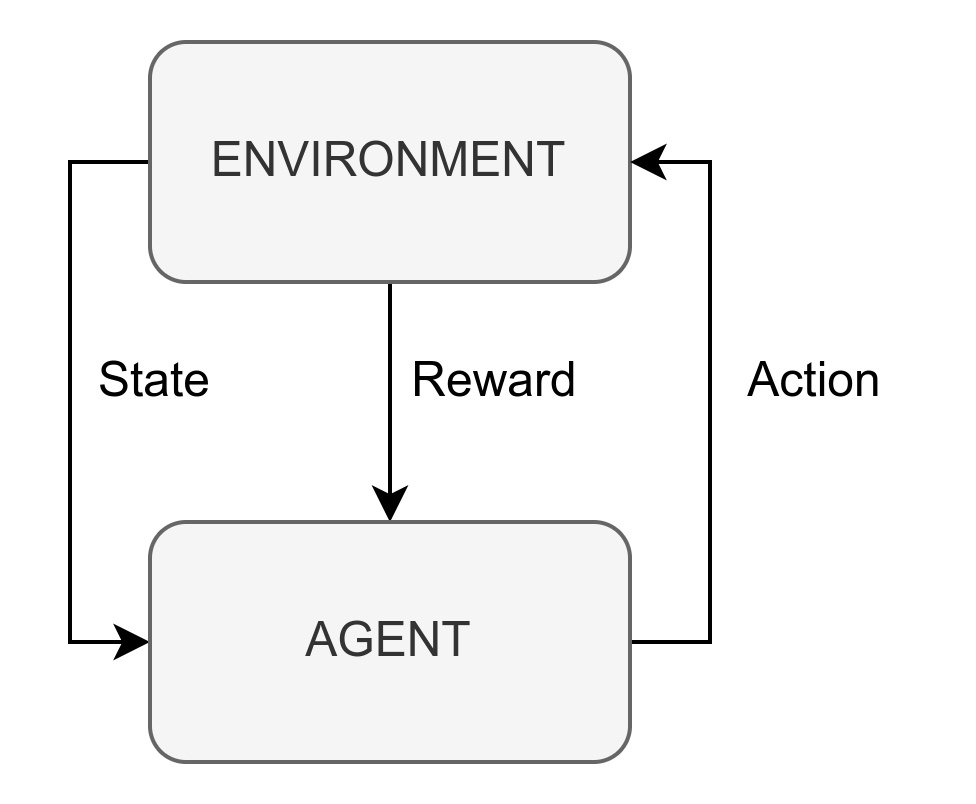
\includegraphics [scale = 0.2]{Images/RL_graph.png}
    \caption{Graph representing reinforcment learning}
    \label{figRL}
\end{figure}
%It can be devided into two strategies for solving said problems. The first strategy involves searching the space or state-action pairs for in order to find which work better in the enviroment. The second technique is estimating the utillity of a particular action. 
The first concept crucial for reinforcment learning is the \textit{reward function} which is objective feedback from the enviroment. It is usually scalar values that are associate with state action pairs. High rewards are usually associate by state-action pairs which benificial for the agent to be situated in whereas negative rewards would then be disadvantageous states or \textit{hazardous} for the agent to be in. Essentially what is good and bad for the agent in the enviroment. The sole objective of the agent is then to maximize this reward\cite{sutton1999reinforcement}.

Naturally we have to define \textit{state} and \textit{action}, which compared to the rest of the concepts have a very general definition. That being the latter is a descision of some sort and the former a factor that has to be taken into considaration when taking an action. 

A central class of methods reinforcment learnign is temporal difference learning. It refers to a class of methods which the learning is based on the difference between temporally successive predictions. It aims to adjust the learner's current expectation for the present input pattern so that it more accurately aligns with the subsequent prediction at the following time step. Unlike Monte carlo methods and other methods in temporal learning updates its estimated value function at every step. \cite{tesauro1995temporal}. 

In temporal learning there are several subcmethods or rather algorithms such as SARSA ,Q learning, TD-Lambda and more \cite{eiben2007reinforcement}. Q learning is an algorithm where the enviroment can be constituted by a controlled Markov process where the agent is controlling it \cite{watkins1992q}. The agent chooses an action and accordingly gets rewarded for it. Q-learning uses the Markov chains to calculate the max reward that can be accumilated by the next state action and updates towards that as shown in the equation below.

\begin{equation} \label{eqQ}
    { Q(s,a) := Q(s,a) + \eta [r + \gamma \max Q(s',a') - Q(s,a)]}
\end{equation}

Equation \ref{eqQ} is the \textit{value} or \textit{update} equation which is responsible for mapping the different states bassed on their estimated long term reward in Q learning. Here $Q(s,a)$ is the current state of the agent $r$ is the reward, $\eta$ is the learning rate and $Q(s',a')$ is the next state. An importnad variable here is $\gamma$ which represent the discount factor. This is used to limit the Markov chain to a limited finite number so they don't end up infinite. This controlls how many steps into the future the agent will try ot estimate. 


\subsection{Genetic Algorithms}

Genteic algorithms are computational models based on the concept of evolution as seen in biology. Similarly to how organisms evolve by natural selection and sexual reproduction, programs can also simulate these processes and behave in a similar fashion to organisms in order to solve a specific problem. In a general sense natural selection is the process which determins which individuals get to survive by some test of fitness. After the best fitted are selelcted the creation or reproduction of the next generation starts. Reproduction is then the method in which the mixing of genes in the remaining population happens and gets passed to the offspring \cite{holland1992genetic}.
\begin{figure}[H]
    \centering
    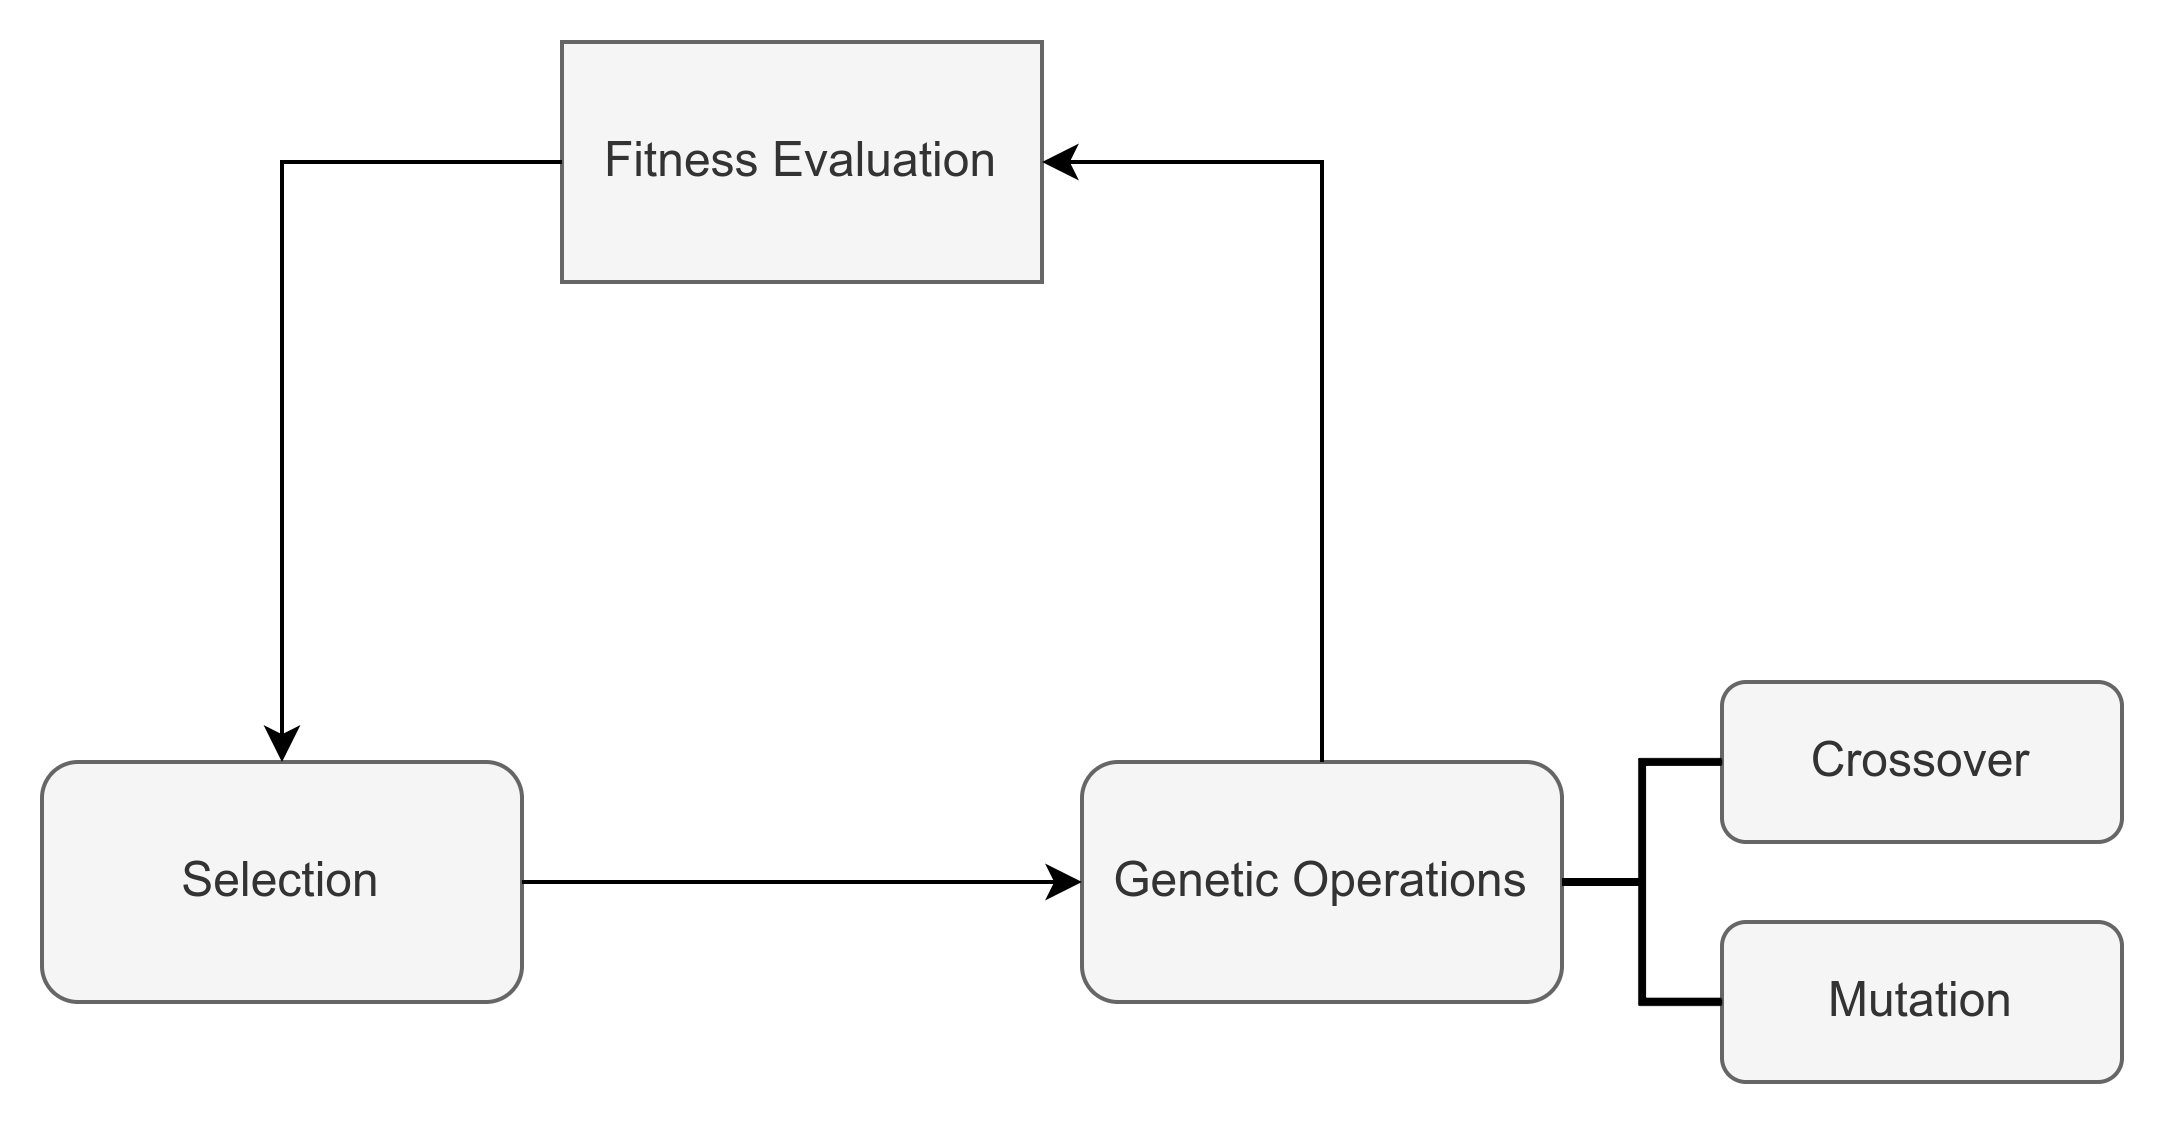
\includegraphics [scale = 0.08]{Images/GA_graph.png}
    \caption{visual representation of genetic algorithms}
    \label{figGA}
\end{figure}

By starting with a population of individuals wich are creaated randomly we have an initial population with variation amongst the individuals. The DNA wich is essentialy the code of the gene can be represented by a string of bits. These string bits can thought as potential solutions to the problem. Due to the variation in the population some individuals vill be better \textit{fit} which then will be selected to remain. In the final stage the remaiining individuals will mix their bit strings to produce individuals for the next generation. These steps will be continually done fore some number of generations \cite{forrest1996genetic}. 

It is importnad however that we reduce the genetic drift and keep track of hte best solutions that have been produced by the previous generation. To do that we employ a method called Elitism. In ellitism compared with traditional reproductiion the most fitting individual are copied to the next generation without any alteration. In that way the best solution of each generation is alway preserved and adds selective preassure and improve convergence speed \cite{du2018elitism}.
% If the theory section is short, you may combine it with the introduction or method section. \par

% This section should provide a short overview of the theoretical background for the experiment. Include all equations (but not elementary/ trivial equations that one can assume the reader knows) that are used in the report. Do not reference the experiment in this section. Rather, write more general and use arbitrary variables in equations (not specific variables for the experiment). \par

% Here are some equations:
% \begin{align} % Use & sign to align, use \nonumber to write a line without number.
%     \laplacian{V} &=0 \nonumber \\
%     \frac{\partial^2 V}{\partial x^2}+\dpd[2]{V}{y} &=0 \label{eq:Laplace} % dpd = display mode partial derivative
% \end{align}

% \Cref{eq:Laplace} % Use \Cref at the start of a sentence and \cref mid sentence.
% is Laplace's equation for electric potentials in two dimensions \parencite[131,136]{Griffiths}. \par
% Here is an example of an equation with different cases:

% \begin{align*} % use equation* or align* to get un-numbered equations.
%     \int_{0}^{a}\sin(nx)\sin(n'x) \dd x = 
%     \begin{cases} 
%         0, \hspace{1cm} \text{if } n'\neq n \\ 
%         \frac{a}{2}, \hspace{1cm} \text{if } n'= n
%     \end{cases}
%     \footnotemark{}
% \end{align*}
% \footnotetext{Notice that the differential operator is \textit{not} italic and that there is a tiny space in front of it.}

% The \verb+NTNU-lab.sty+ includes a some spicy equal signs. For example: 
% \begin{align}
%     \vb{E} & \defeq \frac{\vb{F}}{q} \label{eq:def} \\
%     \vb{E} &\coleq\frac{\vb{F}}{q} \label{eq:col} \\
%     a      &\qmeq b                 \label{eq:qm}  \\
%     G      &\meq \SI{6.6e-11}{m^3 kg^{-1} s^{-2}}  \label{eq:m} 
% \end{align}

% The equality symbols in \cref{eq:def,eq:col} means equal to by definition. Note that these may sometimes be used slightly different from $\triangleq$ (equal to by definition):
% \begin{equation*}
%     a \coleq 3, \hspace{1cm} \Rightarrow \hspace{1cm} a+2 \triangleq 3+2 = 5
% \end{equation*}

% The symbol in \cref{eq:qm} conveys an uncertainty in the statement, as in ``We do not know if $a=b$, but we think it does.'' Such a statement would be followed up by investigating the claim either mathematically or empirically. For example, a paper investigating Ohm's law could state the hypothesis $V\qmeq I\cdot R$ at the start of the paper.\par

% The symbol in \cref{eq:m} is called ``measured by''. Sadly I'm not familiar with how this symbol is used. I can, however, think of two possibilities: \par
% \begin{itemize}
%     \item to define a mathematical object\footnotemark{} by measurement(s) (similar to $\defeq$)
%     \item to specify the measured value of a mathematical object.
% \end{itemize}

% \footnotetext{I used this word as an umbrella term for variables, constants, vectors, tensors and other things that can be measured/ found empirically.}

% \begin{figure}
% \centering
% \begin{circuitikz} \draw
%     (0,0) to[V=15<\volt>] (0,6) to [short, -*, i=50<\milli \ampere>]
%     (2,6) to[R, l=$R_1$] (2,4) 
%     to[R, l=$R_2$] (2,2)
%     to[R, l=${R_3=R_2}$] (2,0) -- (0,0)
%     (2,6) to[short, -*] (4,6)
%     (2,0) -- (4,0)
%     (4,0) to[short, -o] 
%     (4,2)
%     (4.5,1.3) node[label={b}] {}
%     (4,6) to[short,i=$I$,-o] 
%     (4,4)
%     (4.5,4) node[label={a}] {}
%     ;
%     \node[draw,minimum width=1.3cm,minimum height=2cm] at (4,3){Load};
%     \draw [decorate,decoration={brace,amplitude=6pt,mirror,raise=4pt},yshift=0pt]
%     (4.7,2) -- (4.7,4) node [black,midway,xshift=0.8cm] {\footnotesize
%     $R_{\textnormal{Load}}$};
%     \draw[red, thick] (1.5,5.5) rectangle (4.5,6.5)
%     node[pos=0.5, above]{KCL};
%     %\node[] at (2,7){}; % This empty node is used to get some space between the text.

% \end{circuitikz}
% \caption{A circuit diagram. We can apply Kirchhoff's current law (KCL) in the red box and Ohm's law to figure out the unknown values.}
% \label{fig:Circuit}
% \end{figure}

% An example of the first usage would be the gravitational constant, which numerical definition relies on measurements: $G \meq \SI{6.67430(15)e-11}{m^3 kg^{-1} s^{-2}}$.\cite{G_constant} \par
% To give an example of the second way to use the symbol, let us assume you measured a current $I_1$ to be $\SI{3.3(1)}{A}$. Then, you would simply write $I_1\meq \SI{3.3(1)}{A}$, and it would imply that this value was measured (without the need to explicitly mention this in the text). \par
% Personally, I would chose the latter way of using the symbol, simply because this way of using it would occur more frequently in undergraduate reports than the former.
% If you chose to use this symbol, I would recommend clarifying how you use it in a footnote. That is, if its meaning is unclear and/or ambiguous given the context. \par


% \Cref{fig:Circuit} shows a circuit diagram drawn using \verb+circuitikz+. \Cref{tab:Circuit_table} shows possible values for the circuit and is an example of a table with a coloured row. It also shows an example of using footnotes inside tables (normal footnotes inside tables will not be displayed).

% \begin{table}[htb]
%     \centering
%     \begin{tabular}{|c|c|c|}
%          \hline
%          \rowcolor{pink}
%         $R_{\textnormal{Load}}$ & $I$ & $R_1+R_2+R_3$\tablefootnote{This is the same as $2 R_1+R_2$} \\
%         \rowcolor{pink}
%         $(\si{\ohm})$ & $(\si{\milli \ampere})$ & $(\si{\ohm})$ \\
%          \hline
%         350 & 42.9 & 2100 \\
%         400 & 37.5 & 1200 \\
%         500 & 30 & 750 \\
%         1000 & 15 & 428.6 \\
%         1300 & 11.5 & 390 \\
%          \hline
%     \end{tabular}
%     \caption{Some values for the circuit in fig. \ref{fig:Circuit}.}
%     \label{tab:Circuit_table}
% \end{table}
\section{Method}
To evaluate the performance of Reinforcement Learning and Genetic Algorithms,
experiments have been conducted on the simple but effective environment of the cart pole.

Cart Pole is a classic control problem in reinforcement learning. 
The goal is to balance a pole on a cart that can move left or right. 

The state space is four-dimensional, consisting of the cart position, cart velocity, pole angle, and pole angular velocity $[p, v, \alpha, \omega]$. 

The action space is discrete, with two possible actions: move left or move right. 

The reward is 1 for every time step the pole is balanced.

The goal is to balance the pole for as long as possible, with a limit of 500 actions.

The environment, called \textit{CartPole-v1}, is implemented in Python using the Gymnasium library \cite{towers_gymnasium_2023}.
\\
Below described implementations have been trained using the same enviromnemt and ensuring that in every iteration the starting point is the same between two methods, but different from the previous iteration, to ensure that the comparison can be evaluated \textcolor{blue}{without considering the stochastic nature of the training}.

\subsection{Reinforcement Learning}
The reinforcement learning implementation is based on temporal differenc learning \cite{sutton1998temporal}, 
in particular Q-learning.
The implementation takes inspiration on the work of \textit{JackFurby} \cite{JackFurbyCartPole}.

The \textit{Q-table} is represented by the discretization of the continuous 4-dimensional state vector in 20 even intervals for every dimension of the vector leading to 160000 possible pairs of $<state,action>$, considering the two possible actions.

\begin{figure}[H]
	\centering
	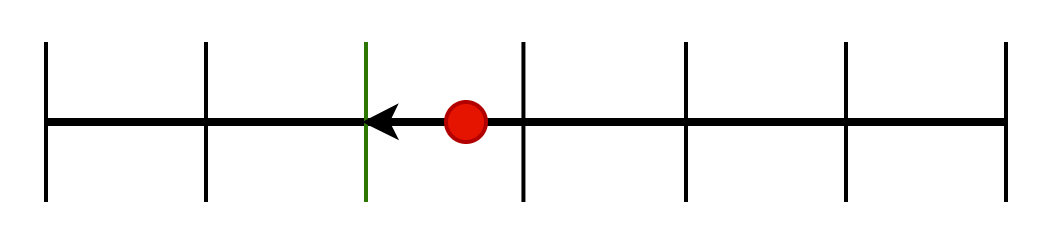
\includegraphics [scale = 0.2]{Images/state_discretization.png}
	\caption{Representation of the state discretization technique, considering an element of the 4D-state, $s_i$, the red dot is the real value of $s_i$, this is discretized to the nearest leftwise discrete state.}
	\label{figDISC}
\end{figure}

Once an action is performed, the state selected is the first larger that the observed state.\\
The parameters used in the experiments are the following:


\begin{table}[htb]%
	\centering
	\label{tab:RL_parameters}
	\begin{tabular}{|S|S|} 		% S = special column format from the siunitx package. Aligns commas.
		
		\hline
		{\textbf{Learning rate $\alpha$}} &  {0.1} \\
		\hline
		{\textbf{Discount factor $\gamma$}} & {1} \\
		\hline
		{\textbf{Number of episodes $n_{ep}$}} & {20000} \\
		\hline
		{\textbf{Exploration rate $\varepsilon$}}  & {variable} \\
		\hline
		{\textbf{Mutation Rate}} & {0.05} \\
		\hline
		{\textbf{Penalty factor $PF$}}& {-375} \\
		\hline
		
	\end{tabular}
	\caption{Parameters used in the RL implementation. The exploration rate $\varepsilon$ starts with $\varepsilon(0)=1$ and decays by $\varepsilon(t) = \varepsilon(t - 1) - \frac{1}{\frac{n_{ep}}{2} - 1}$, every episode, stopping after $\frac{n_{ep}}{2}$ episodes. }
\end{table}



\subsection{Genetic Algorithms}

\textbf{Genotype}\\
Since Genetic Algorithms can be very different depending on the genotype chosen to represent individuals, we have tried several different implementation of GA, varying the used genotype.
\\

\subsubsection{Encoding the sequence of actions}
The first method used is a very naive implementation that can be applied to a very large variety of problems with GA : reprensenting individuals with the vector of all actions they will perform in order.
Thus, \textit{i-th} character of the genotype of an individual $j$ corresponds to the \textit{i-th} action performed by the corresponding individual.
In this apporach, mutation is performed by switching an action in the genotype from left to right or from right to left with a probability given by the \textit{Mutation rate} for every action $i$ inside the genotype.
\\
Since this particular genotype does not generalize well with the random initialization of the starting position of the pole. Due its intrinisc dependecy with the initial state, fixed starting conditions should be applied to effectively train in a meaningful way this genotype, by seeding the environment to always start in the same place, but this leads to a scarse ability of generalization, since the training is valid just for a determinated starting position of the pole.

All those considerations lead to the decision of evaluating other encodings for the final implementation.\\
\subsubsection{Encoding a state-action table}
The second encoding takes inspiration from Reinforcement Learning \textit{Q-table}.
In this approach, the focus is not to predict every action one by one  but instead use GA to assign values to state-actions pairs then select the action that referes to the observed state.\\
The discretization techninque is the same used in the reinforcement learning implementation and briefly described in figure \ref{figDISC}.\\
Here, mutation is performed by swapping the action of a given state with a probability given by the \textit{Mutation rate}.
\\

\textbf{Parameters}\\
The GA parameters can be found in the following table :
\begin{table}[htb]%
	\centering
	\caption{Parameters used in the GA implementation}
	\label{tab:GA_parameters}
	\begin{tabular}{|S|S|} 		% S = special column format from the siunitx package. Aligns commas.
		
		\hline
		{\textbf{Genotype}} &  {Q-table} \\
		\hline
		{\textbf{Population Size}} & {100} \\
		\hline
		{\textbf{Generations}} & {200} \\
		\hline
		{\textbf{Selection}}  & {Fitness} \\
		\hline
		{\textbf{Mutation Rate}} & {0.005} \\
		\hline
		{\textbf{Crossover}}& {one-point} \\
		\hline
		{\textbf{\textcolor{blue}{Elitism}}}& {\textcolor{blue}{2} } \\
		\hline

	\end{tabular}
\end{table}



\section{Results}

\subsection{Training comparison}

The training phase of a Reinforcement Learning agent and a Genetic Algorithm are fundamentally different.
Therefore, a way to harmonize the training data of the two methods in order to compare them has to be found.
\\
The first modification is to consider RL episodes the same as GA individuals and aggregate the RL performances to match the number of generations used for GA.
For example considering a population size of $k$ for the Genetic Algorithm, the max and mean of every $k$ Reinforcement Learning episodes have been considered to compare them with each GA generation. Here, $k$ = 100.
\\
Second, the runtime per iteration might not be the same between the two methods. To account for this difference, the performance data was plotted not against the number of iterations but against the training time (in seconds).
Of course both algorithms were ran on the same machine for a fair comparison.
\\
Figure \ref{figAVG} and Figure \ref{figMAX} show both average and best results achieved over training time for our two methods.

\begin{figure}[H]
	\centering
	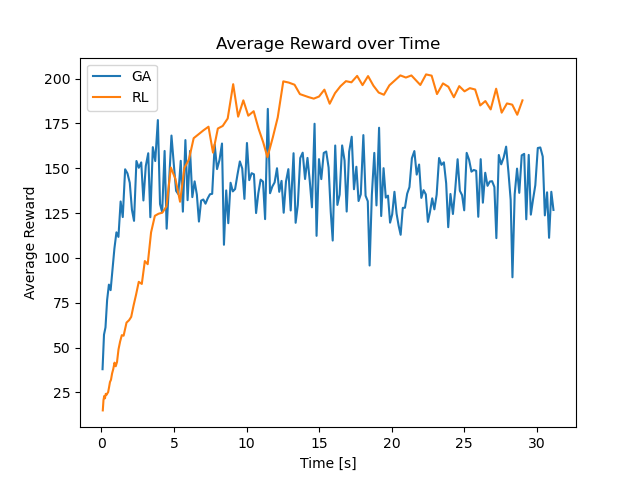
\includegraphics [scale = 0.5]{Images/RL_GA_comparison_avg.png}
	\caption{Evolution of mean score in time of both the two algorithms.}
	\label{figAVG}
\end{figure}

\begin{figure}[H]
	\centering
	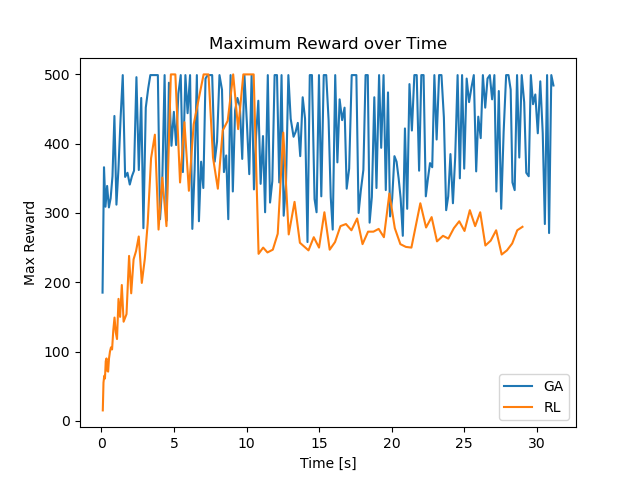
\includegraphics [scale = 0.5]{Images/RL_GA_comparison_max.png}
	\caption{Evolution of max score in time of both the two algorithms.}
	\label{figMAX}
\end{figure}

As can be seen in Figure \ref{figAVG} and Figure \ref{figMAX}, the first takeaway is that RL scores much better than GA.
One interesting point though, is that GA performances seem to grow quicker than their RL counterpart at the beginning of training.
This can be explained by the fact that GA performs parallel search and that the genotype can be modified much more in one crossover than RL's Q-table in an episode. 
These two factors create more variety in the achieved solutions and by retaining the best out of them, it is easy to see how we might arrive earlier to a viable solution.
\\
However, the other side of this described coin is that, with less stability provided by GA, comes a harder time in making specific and iterative changes to a solution.
Looking at Figure \ref{figAVG}, it is very interesting to note these very similar performances between the two algorithms at 10 to 20 seconds of training, before RL jumps much higher while GA keeps plateau-ing at the same level.
An explanation to the phenomenon might be that RL iteratively tweeks the same solution to perform better which allows to fix encountered problems. Meanwhile, GA might provide too much change over each generation to slowly improve an existing solution further, explaining the flattening out of performance.

\subsubsection{Angle magnitude difference.}
Another difference between the two approach is the behavior of the agent during the game itself.
This was only made visible once GIFs were generated to view sample games, as resumed in Figure \ref{fig:framesRL} for the reinforcement learning agent and Figure \ref{fig:framesGA} for the genetic algorithm last generation. 
It became apparent that the RL trained agent was taking way wider swings and generally playing more "on the edge" than the GA trained agent who is keeping the pole more straight and moving more cautiously.
This initial obsevation was confirmed more quantitatively, by measuring the average absolute value of the angle of the pole during every episode of training.
Indeed, it turns out that the average absolute value of the angle is consistently two orders of magnitude greater during RL training than during GA training.
Since it doesn't penalize exploratory moves, Q-Learning specifically is known to be more prone to taking risks than other RL techniques. However, we tried using SARSA (another RL method without this feature) and still confirmed the same results.
\\
This last remark might be even more surprising considering that we know the RL agent clearly outperforms the Genetic Algorithm, we might intuitively think that keeping the pole more straight would reflect better overall play.


% GA FRAMES %

\begin{figure}[H]
	\centering
	\begin{subfigure}
		\centering
		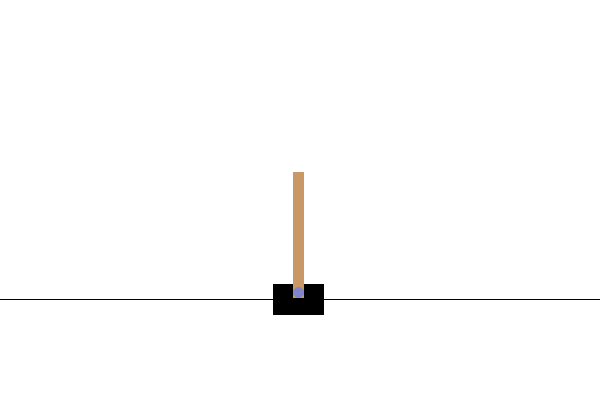
\includegraphics[width=0.3\linewidth]{Images/frames/GA/6.png}
	\end{subfigure}
	\hfill
	\begin{subfigure}
		\centering
		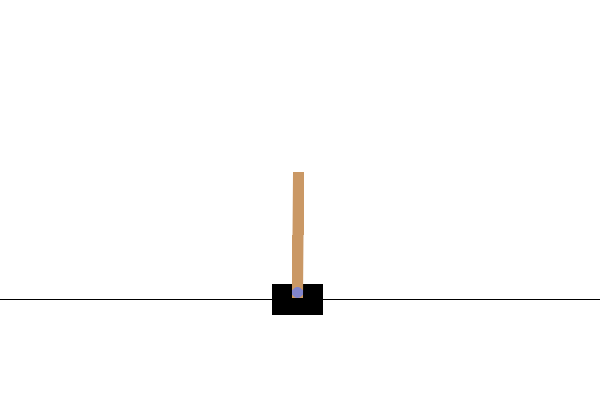
\includegraphics[width=0.3\linewidth]{Images/frames/GA/9.png}
	\end{subfigure}
	\hfill
	\begin{subfigure}
		\centering
		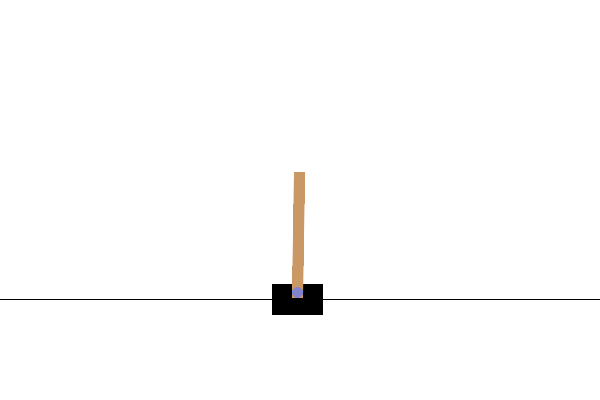
\includegraphics[width=0.3\linewidth]{Images/frames/GA/12.png}
	\end{subfigure}
	\\
	\begin{subfigure}
		\centering
		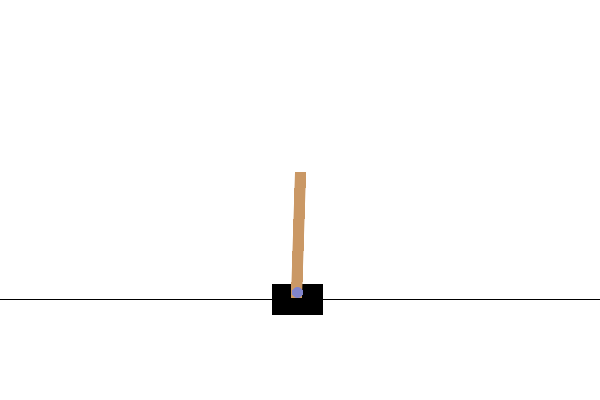
\includegraphics[width=0.3\linewidth]{Images/frames/GA/15.png}
	\end{subfigure}
	\hfill
	\begin{subfigure}
		\centering
		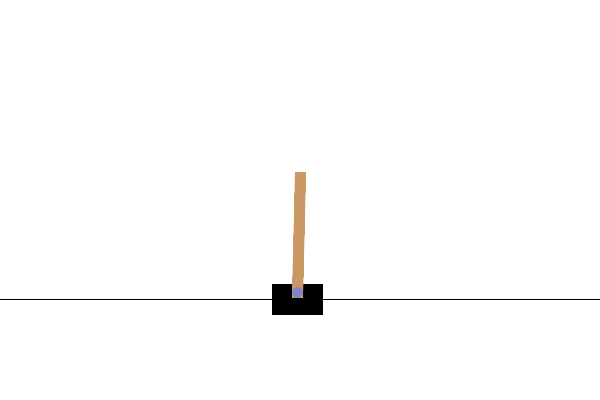
\includegraphics[width=0.3\linewidth]{Images/frames/GA/18.png}
	\end{subfigure}
	\hfill
	\begin{subfigure}
		\centering
		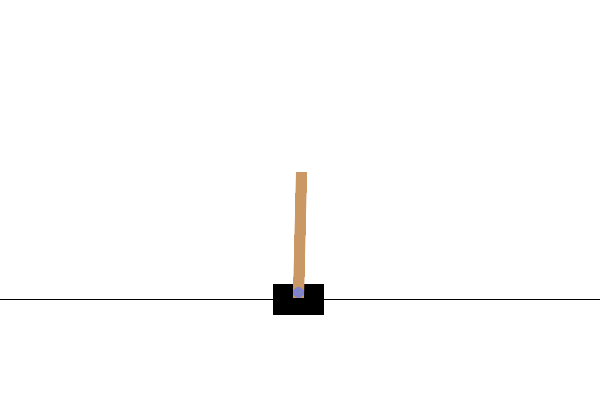
\includegraphics[width=0.3\linewidth]{Images/frames/GA/21.png}
	\end{subfigure}
	\caption{6 early frames of a game played by the Genetic Algorithm last generation, as can be seen the agent is keeping the pole straight with very little movement.}
	\label{fig:framesGA}
\end{figure}

% RL FRAMES %
\begin{figure}[H]
	\centering
	\begin{subfigure}
		\centering
		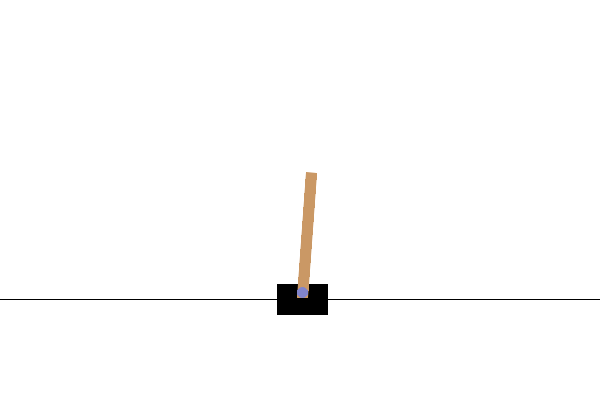
\includegraphics[width=0.3\linewidth]{Images/frames/RL/6.png}
	\end{subfigure}
	\hfill
	\begin{subfigure}
		\centering
		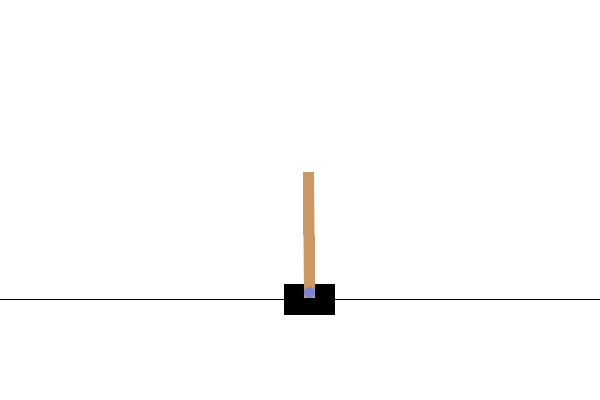
\includegraphics[width=0.3\linewidth]{Images/frames/RL/9.png}
	\end{subfigure}
	\hfill
	\begin{subfigure}
		\centering
		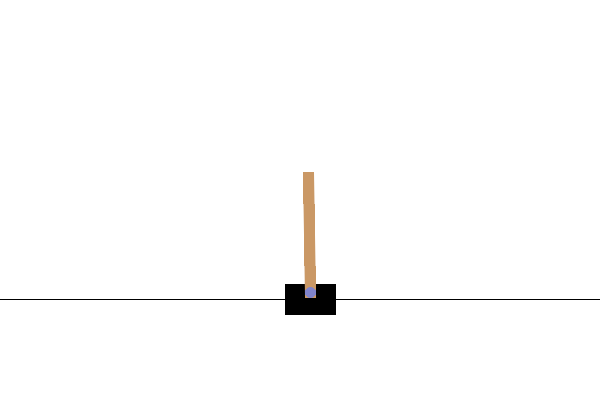
\includegraphics[width=0.3\linewidth]{Images/frames/RL/12.png}
	\end{subfigure}
	\\
	\begin{subfigure}
		\centering
		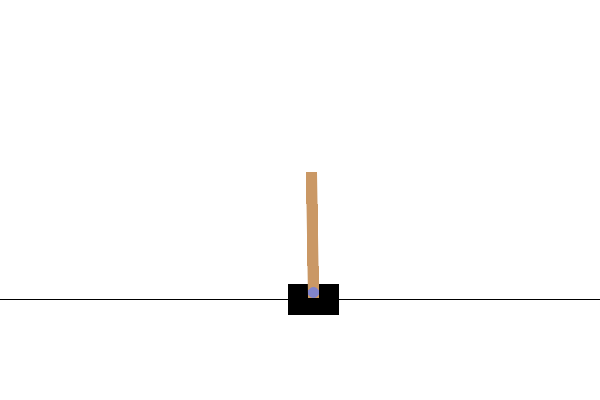
\includegraphics[width=0.3\linewidth]{Images/frames/RL/15.png}
	\end{subfigure}
	\hfill
	\begin{subfigure}
		\centering
		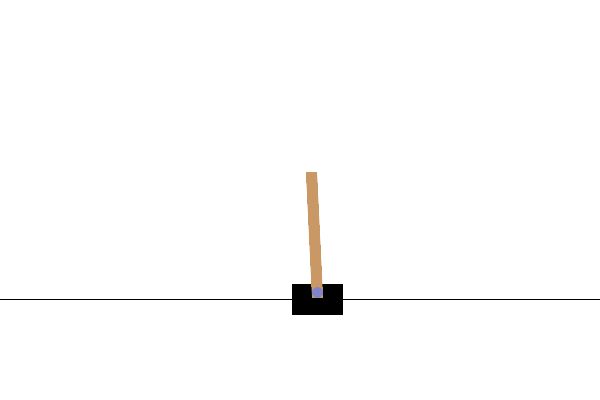
\includegraphics[width=0.3\linewidth]{Images/frames/RL/18.png}
	\end{subfigure}
	\hfill
	\begin{subfigure}
		\centering
		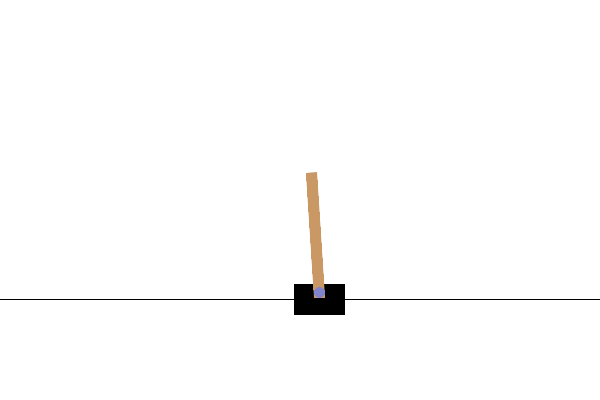
\includegraphics[width=0.3\linewidth]{Images/frames/RL/21.png}
	\end{subfigure}
	\caption{6 early frames of a game played by the Reinforcement Learning agent, as can be seen the agent is taking wider swings and playing more "on the edge" than the GA trained agent.}
	\label{fig:framesRL}
\end{figure}

\textit{Since displaying one image every frame is very little change and hard to observe without showing too many of them at once, the images above are picked every 3 frames of a played game.
They are Respectively frames number 6, 9, 12, 15, 18 and 21.}

\subsection{final model comparison}

The second approach used to compare the obtained results is based on the final models' observations.

\subsubsection{State-Action table}

Figure \ref{figTABLEDIFF} shows the difference between the two obtained state-action tables of the final reinforcement learning agent and one of the individuals from the last generation of the genetic algorithm.

Since the \textit{Q-Table} does not provide an exact chosen action given a state, the compared state-action table of the reinforcement learning agent used in Figure \ref{figTABLEDIFF} is obtained by selecting the action $a$ of the state $s$ based on $argmax_{a_i} (Q(s,a_i))$.

\begin{figure}[H]
	\centering
	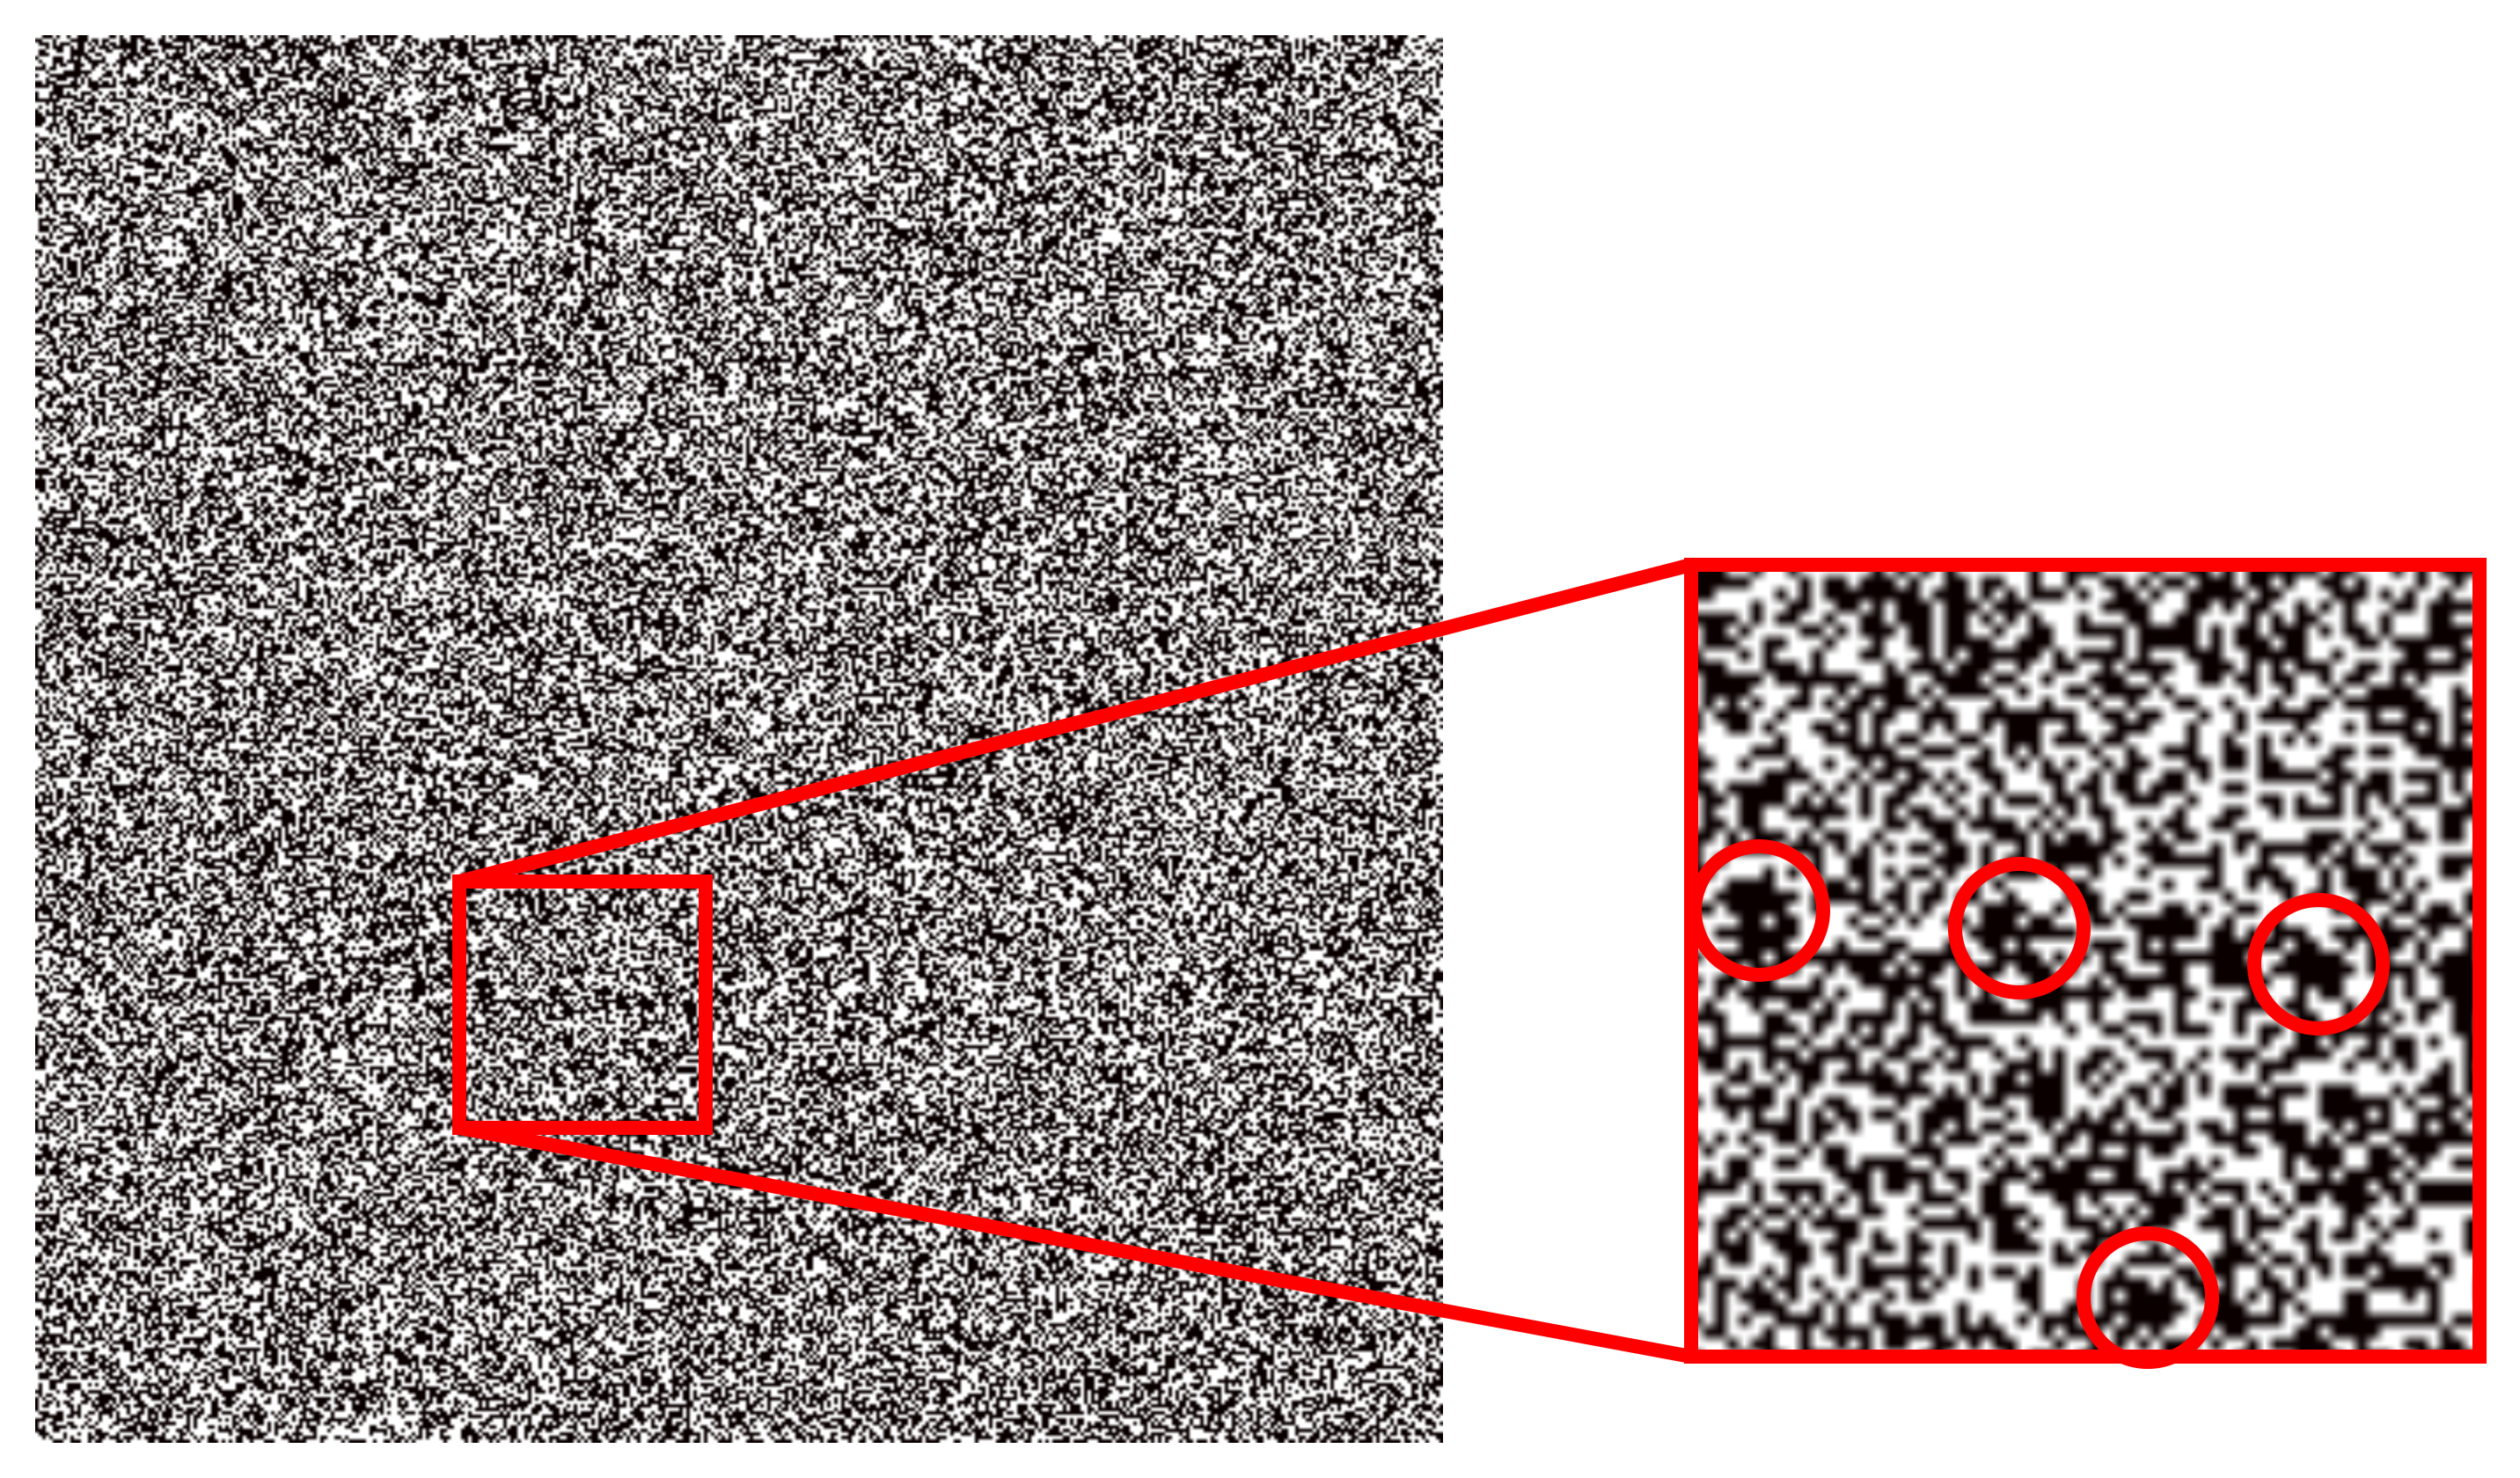
\includegraphics [width=\linewidth]{Images/diff_zoomed.png}
	\caption{Difference between the two state-action tables obtained using GA and RL. The black pixels represent the states where the chosen action is the same, while white pixels represent a different action choice. The x-axis contains all the possible pairs of the first two elements of the state's vector, $(s_1,s_2)$, and the y-axis contains all the possible pairs of the last two elements, $(s_3,s_4)$. }
	\label{figTABLEDIFF}
\end{figure}


Looking into Figure \ref{figTABLEDIFF}, it is possible to observe how the actions selected by the two algorithms differ in various states. However, some wide areas where the action taken by both algorithms is the same can be spotted, which could be referred to as sensitive states where considering a different choice could lead the pole to fall down.\\

\begin{figure}[H]
	\centering
	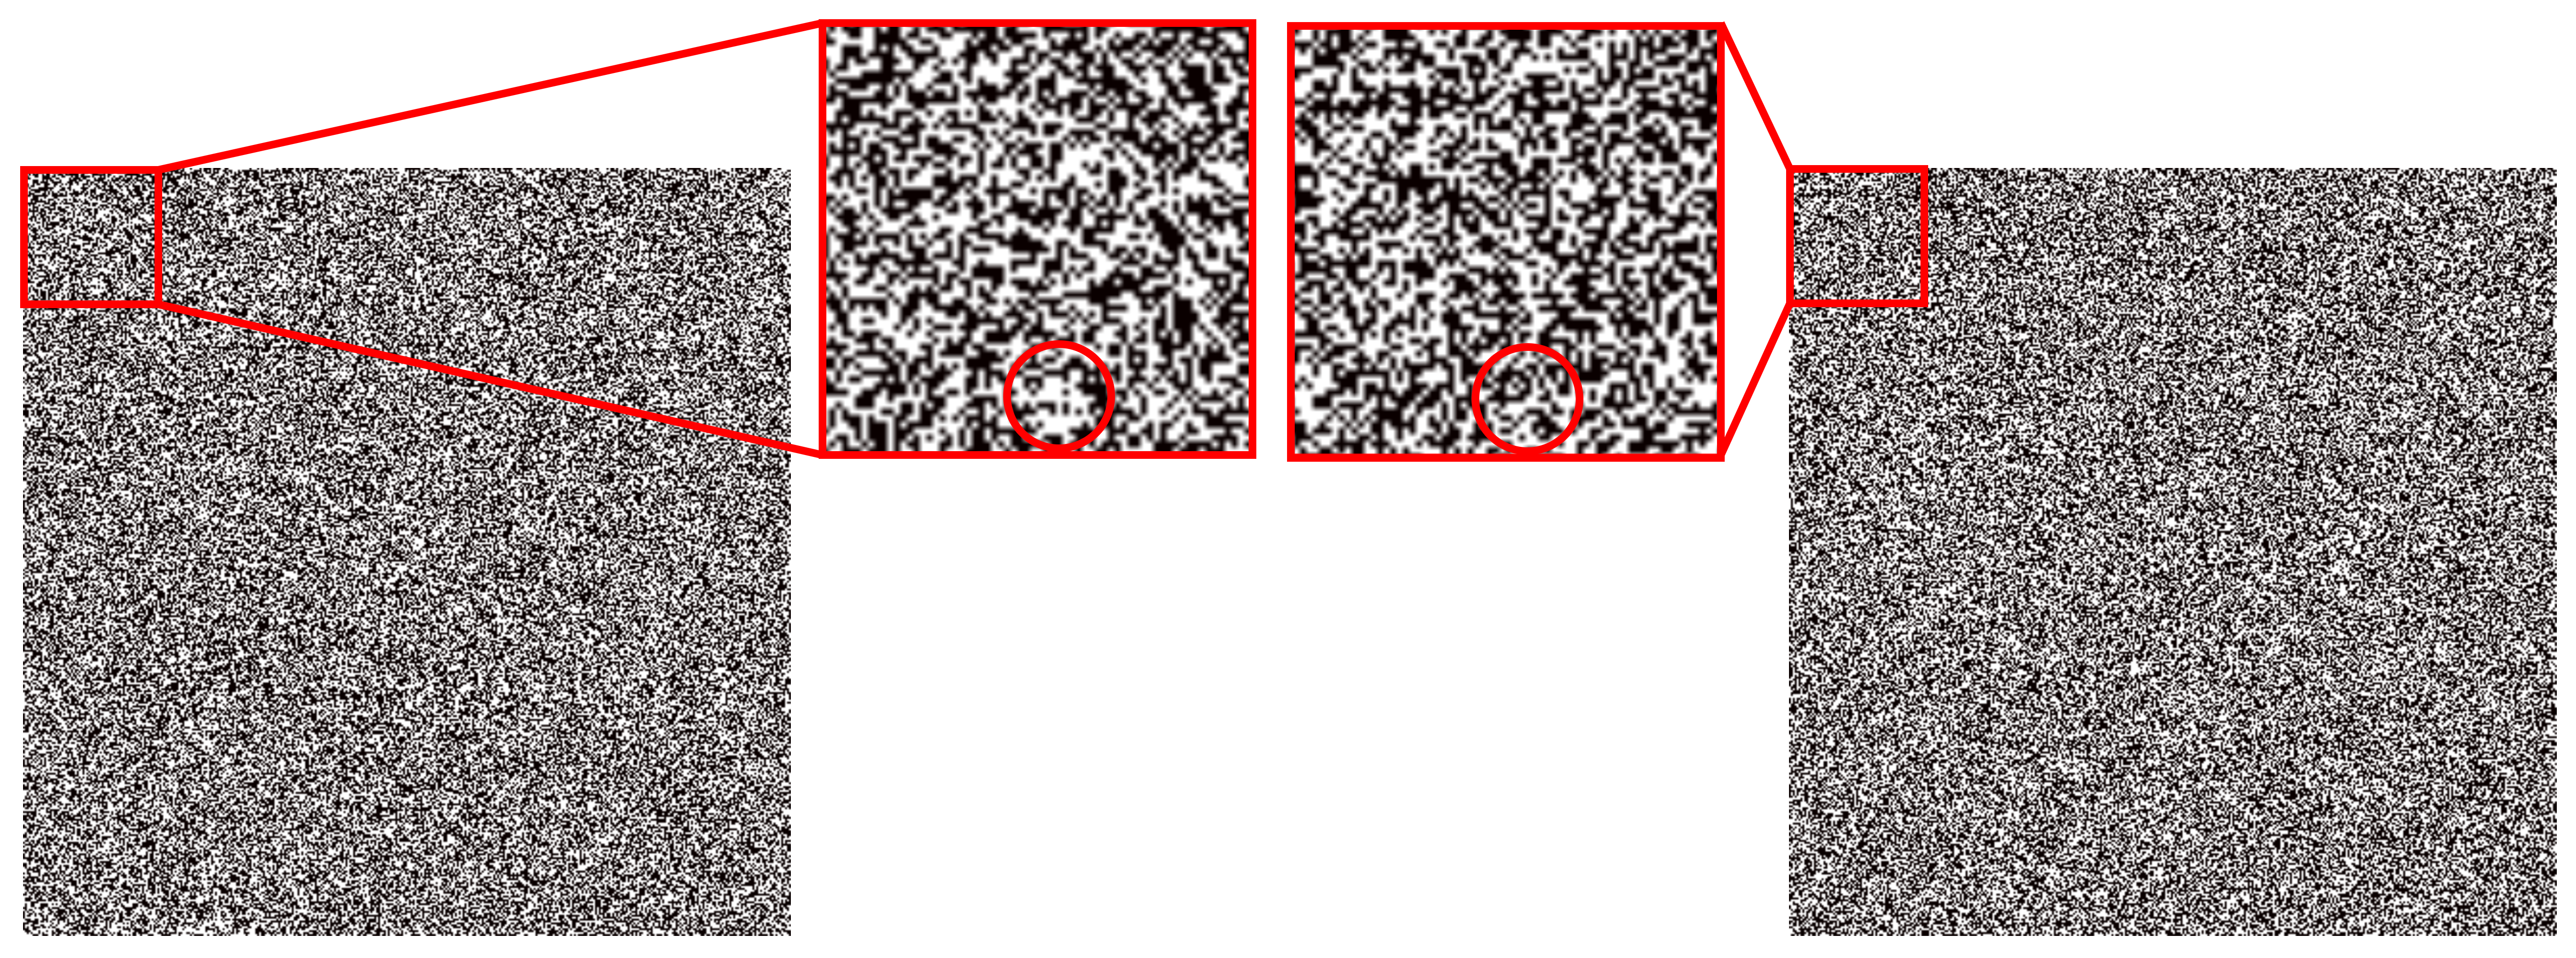
\includegraphics [width=\linewidth]{Images/diff_comparison.png}
	\caption{Evolution of the state-action table of both models: on the left, the differences of the final state-action table, on the right, the differences among the state-action table on the two models before the training.}
	\label{figDIFF_COMPARISON}
\end{figure}


Figure \ref{figDIFF_COMPARISON} shows the evolution of the state-action table of the two models, before and after the training. The resulting table differes in several points from the starting one, Figure \ref{figDIFF_COMPARISON} highlights one section where the two algorithm decided to performed the opposite actions. 

\subsubsection{Testing performances}

Figure \ref{figRLvsGA} shows the final testing results of the two methods. As already showed by the traning comparison in both figure \ref{figAVG} and figure \ref{figMAX}, The reinforcement learning agent showed a better generalization ability and more understanding of the environment, leading to obtain better results.\\
The testing has been conducted as follow: the environment has been seeded with ten different seeds and for every execution the same environment has been provided to both the algorithm.
The reinforcement learning agent has been tested using the obtained \textit{q-table} from the training, the genetic algorithm population is the last generation of the training performed.\\
Every individual of the GA population have been tested for all the tests, and the best one has been considered for the comparison, during the testing of the population, no particular difference have been noticed between the reward obtained by the individuals.

\begin{figure}[H]
	\centering
	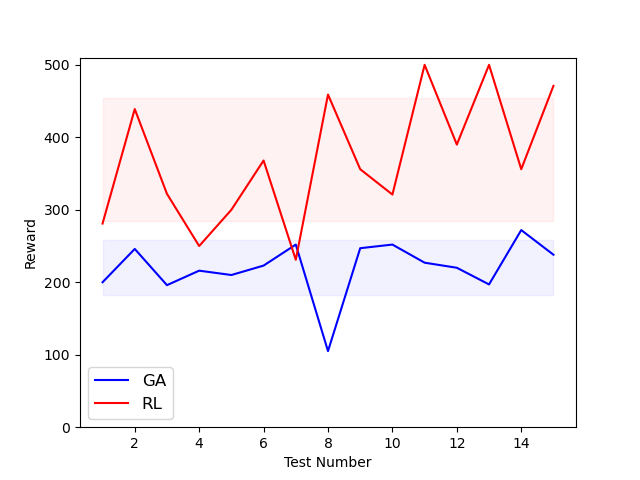
\includegraphics [width=0.5\textwidth]{Images/RL_vs_GA.png}
	\caption{The plot shows the results obtained testing the two models on the same test set. The x-axis represents the number of the test set, the y-axis the number of steps the model was able to take before reaching the goal. The blue line represents the results obtained using the model trained with the GA, the red line the results obtained using the model trained with the RL.}
	\label{figRLvsGA}
\end{figure}

Observing the results, some differences regarding the variance can be noticed: the GA population seem to obtain more consistent results in different tests, but due the fact that the testing is performed on the entire generation this could be related to the fact that every time the best individual is extracted.\\


	



% % Delete the text and write your Results here:
% %------------------------------------

% The results section can be combined with the discussion if appropriate. In case of many sub\-/experiments % \-/ fixes the problem that LaTeX won't hyphenate words with dashes in them.
% where the results are vaguely related or unrelated, it would be appropriate to combine the results and discussion. This way you have the information related to each sub-experiment gathered in one place. \par
% Provide uncertainties for the results, but don't discuss it. Do not involve personal opinions, just present the cold hard results in form of numbers, tables, graphs and some sentences. \par
% \Cref{tab:Some-numbers} shows a nice table with comma alignment. \par

% \begin{table}[htb]%
% \centering
% \caption{Table with comma alignment.}
% 	\label{tab:Some-numbers}
% 	\begin{tabular}{SSS} 		% S = special column format from the siunitx package. Aligns commas.
% 		\toprule
% 		{$m$}  &  {$a$}  & {$F$}  \\
% 		{(\si{kg})} &  {(\si{m.s^{-2}})} & {(\si{N})}  \\
% 		\midrule
% 		1,2 & 10,1 & 12 \\
% 		2,44 & 6,92 & 16,88 \\
% 		10 & 1,0 & 10 \\
% 		8,2 & 1,1 & 9,0 \\
% 		100 & 1 & 100 \\
% 		\bottomrule
% 	\end{tabular}
% \end{table}


\section{Related Works}

% add sources
Similar comparisons between RL and GA have been made by \cite{drugan2019reinforcement},\cite{taylor2006comparing} and \cite{pollack1997coevolution}. \cite{drugan2019reinforcement}  focuses more on a comprehensive overview of recent trends in the field rather than comparing subclasses of algorithms or particular aspects of RL and GA and states that both can be good at solving RL problems. \cite{pollack1997coevolution} successfully trained an evolutionary algorithm to play backgammon, a typical RL type game. \cite{moriarty1996efficient} presents a reinforcement learning technique SANE((Symbiotic, Adaptive Neuro-Evolution)) which uses a genetic algorithm to evolve a population of neurons to perform a task. The evaluation which was done using the inverted pendulum problem in the form of a cart pole. Using the same problem it was compared to Q learning and was found to be 2 times faster. Several works focus on combining these two methods for machine learning by either using GA to train RL or vice versa such as \cite{eiben2007reinforcement} where the authors try to use Reinforcement learning to tune the parameters of GA.  Papers such as  \cite{khadka2018evolutionary} explore the opposite combination of training RL using GA . It is important to mention that the implementation of the reinforcement learning algorithm that is used is based on the work of \textit{JackFurby} \cite{JackFurbyCartPole}. 

In our investigation into various genotype options for addressing the pole-balancing problem, we consciously opted not to explore a solution based on NEAT\cite{stanley2002NEAT} networks, build a neural network able to predict the correct action given the environment state as input.\\
Considering the simplicity of the chosen environment and given our primary objective of comparing genetic algorithm (GA) approaches with reinforcement learning (RL) agents, we excluded the possibility to employ a NEAT network for such environment.

Ensuring a fair and transparent comparison between GA and RL methods is the main objective. Introducing unnecessary complexity through a NEAT network could potentially obscure the true comparative performance of the two approaches. Thus, we chose simpler solutions, aligning more closely with typical RL agent implementations. This approach facilitates a clearer evaluation of the relative effectiveness and efficiency of GA and RL algorithms in the pole-balancing task.
\section{Discussion}
% Delete the text and write your Discussion here:
%------------------------------------

You should try to show insight into what happened and why, and how things could have
gone differently. If you have presented any background theory, try to tie it together with
your results. How do they relate? If they differ, try to explain why. Even if things didn’t
work out as intended, a good discussion shows that you’ve understood what went wrong
and how you could potentially overcome these obstacles. 
\section{Conclusion}
% Delete the text and write your Conclusion here:
%------------------------------------

The experiments concluded that Genetic Algorithms can be an interesting pathway to parametrize features inspired from Reinforcement Learning (here the \textit{Q-table}).
However RL still vastly outperforms GA on the studied task, supposedly due to the precision required to improve pole balancing and a very large hyper-parameters search space.
GA may thus be better suited (and possibly outperform RL) on tasks with a larger search space or requiring less precision, where its parallel search could allow it to converge to a viable solution faster while not being impaired by its "blind" update steps.

%The conclusion should summarise your main results and main points from the discussion.
%A rule of thumb is to not present any new information (information not found in the results or discussion).
%\clearpage                                     % Sometimes you want the rest on separate pages.
\section*{Acknowledgements}
% Delete the text and write Acknowledgements here (not required, can be omitted):
% Comment out ' \section*{Acknowledgements}
% Delete the text and write Acknowledgements here (not required, can be omitted):
% Comment out ' \section*{Acknowledgements}
% Delete the text and write Acknowledgements here (not required, can be omitted):
% Comment out ' \input{Text/Acknowledgements} ' to remove this section.
%------------------------------------


Acknowledgements (nb. takksigelser, nn. takkseiingar) is not a requirement in a laboratory report. However, it is used in most 
scientific articles. It looks more professional and adds some ``extra spice'' to your report. Here is an example: \par
The authors would like to thank Dr. Ola Normann at the
University of Oslo for assistance with the SIMS-analysis
and Dr. Kari Normann at NTNU for fruitful discussions
and support concerning melt spinning of silicon. This work
was financially supported by the Norwegian research council and the Norwegian PhD Network on Nanotechnology
for Microsystems.
 ' to remove this section.
%------------------------------------


Acknowledgements (nb. takksigelser, nn. takkseiingar) is not a requirement in a laboratory report. However, it is used in most 
scientific articles. It looks more professional and adds some ``extra spice'' to your report. Here is an example: \par
The authors would like to thank Dr. Ola Normann at the
University of Oslo for assistance with the SIMS-analysis
and Dr. Kari Normann at NTNU for fruitful discussions
and support concerning melt spinning of silicon. This work
was financially supported by the Norwegian research council and the Norwegian PhD Network on Nanotechnology
for Microsystems.
 ' to remove this section.
%------------------------------------


Acknowledgements (nb. takksigelser, nn. takkseiingar) is not a requirement in a laboratory report. However, it is used in most 
scientific articles. It looks more professional and adds some ``extra spice'' to your report. Here is an example: \par
The authors would like to thank Dr. Ola Normann at the
University of Oslo for assistance with the SIMS-analysis
and Dr. Kari Normann at NTNU for fruitful discussions
and support concerning melt spinning of silicon. This work
was financially supported by the Norwegian research council and the Norwegian PhD Network on Nanotechnology
for Microsystems.
                   % Comment out to exclude the Acknowledgements section

%%%%%%%%%%%%%%%%%%%%%%%%%%%%%%%%%%%%%%%%

% Bibliography
%--------------------
\printbibliography

%\clearpage                                     % Sometimes it is useful to have appendix on separate page.
%\onecolumn                                     % If you want 1 column for appendix.
\appendix
% Delete the text and write Appendix here (not required, can be omitted):
% Comment out ' \appendix
% Delete the text and write Appendix here (not required, can be omitted):
% Comment out ' \appendix
% Delete the text and write Appendix here (not required, can be omitted):
% Comment out ' \input{Text/Appendix} ' to remove this section.
%------------------------------------


\section{Additional Information}

You can use the appendix to include information that is relevant, but does not belong in the report. In most cases however, the appendix can be omitted and isn't necessary. \par
\subsection{Python code}
If you used python code to process data, you can include the code (or a shorter version of it) in the appendix. Usually, however, it is better to hand in a separate file containing your code together with the report.
\appendixfootnote{Rule of thumb: short code goes in the appendix, long code goes in a separate file} \par

Below is a simple example of some code used to calculate the values for the circuit in \vref{fig:Circuit} 
% because I have loaded varioref and cleveref (in that order) varioref has "become clever", and you can
% use \Vref{} in the start of a sentence.
\appendixfootnote{exaple usage of the varioref package}
found in \cref{tab:Circuit_table}:

\begin{listing}[!htb]

\inputminted[%
firstline=7, 
lastline=14,
bgcolor=LightGray,
breaklines,
breaksymbolleft={},
breakindent={15pt}
]{python}{Code/Python/Circuit_Calculation.py}

\caption{Example from external file}
\label{listing:1}
\end{listing}

The code from \cref{listing:1} was displayed using a \verb+.py+ file. Since the lines are not numbered in this code example, you can copy and paste the code from the PDF into python without many issues (does however need to correct indents). \par
I would advice against using the \verb+lstlisting+ package to display code, as this introduces many unnecessary problems when trying to copy-paste the code.\par

\section{Appendix footnotes}
This template has a separate roman numeral footnote system for the appendix. You can chose to use this or normal footnotes in the appendix. Use the command \verb+\appendixfootnote{text}+\appendixfootnote{Note that there is \textbf{no} commands: \textbackslash appendixfootnotemark and \textbackslash appendixfootnotetext} to get a (lower case) roman numerical footnote. I added this footnote system because I thought it would be nice to have a separate footnote system for the appendix, since this section is in some ways separate from the rest of the document.

\section{Boxes}
This template also include two box environments to highlight text. I will showcase these in the two next subsections.

\subsection{Info Box}
The first environment is named \verb+infobox+ and is numbered, which allows for references to the box. You can also change the title of the box as well as the colours. To change the colour use the command \verb+\SetInfoBoxBgColor{}+ (changes background colour) and \verb#\SetInfoBoxFrameColor{NTNU_blue}# (changes frame colour). The default colours are a light blue background and a darker blue frame. Here is an example:

\begin{infobox}[label=box:info]{Infobox}
Here is an infobox. You can also write math inside it:
\begin{align*}
    3x+5y=6z^2
\end{align*}

\end{infobox}

Here is a reference to the infobox: \cref{box:info}. Notice that the structure of the infobox numbering is (section number)-(box number). The first infobox in section 2 thus has the reference 2-1.

\subsection{Simple Box}
The second environment is just a coloured box with no number or title. This can be used just to highlight text. \par
I also added a theorem environment \verb?Sclaw? that may prove useful. 

\begin{simplebox}
\begin{Sclaw}[Newton's 2. law]
\label{law:N2}
$\vec{F}=\frac{\dd \vec{p}}{\dd t}$
\end{Sclaw}
\end{simplebox}
You can reference the theorem environment: See \cref{law:N2}. I also added a Norwegian version of the environment: \verb+naturlov+.
Let us change the colour of the next box to blue using \verb?\SetSimpleBoxColor{bg_blue}?.

\SetSimpleBoxColor{bg_blue}
\begin{simplebox}
To create your own theorem environment, use the command \verb?\newtheorem{}{}[]?.
\end{simplebox}

You must use the \verb+newtheorem+ command before \verb?\begin{document}? (the preamble). You can read more about the theorem environment in the \href{https://www.overleaf.com/learn/latex/Theorems_and_proofs}{Overleaf documentation} using this link:\\ \url{https://www.overleaf.com/learn/latex/Theorems_and_proofs}.
 ' to remove this section.
%------------------------------------


\section{Additional Information}

You can use the appendix to include information that is relevant, but does not belong in the report. In most cases however, the appendix can be omitted and isn't necessary. \par
\subsection{Python code}
If you used python code to process data, you can include the code (or a shorter version of it) in the appendix. Usually, however, it is better to hand in a separate file containing your code together with the report.
\appendixfootnote{Rule of thumb: short code goes in the appendix, long code goes in a separate file} \par

Below is a simple example of some code used to calculate the values for the circuit in \vref{fig:Circuit} 
% because I have loaded varioref and cleveref (in that order) varioref has "become clever", and you can
% use \Vref{} in the start of a sentence.
\appendixfootnote{exaple usage of the varioref package}
found in \cref{tab:Circuit_table}:

\begin{listing}[!htb]

\inputminted[%
firstline=7, 
lastline=14,
bgcolor=LightGray,
breaklines,
breaksymbolleft={},
breakindent={15pt}
]{python}{Code/Python/Circuit_Calculation.py}

\caption{Example from external file}
\label{listing:1}
\end{listing}

The code from \cref{listing:1} was displayed using a \verb+.py+ file. Since the lines are not numbered in this code example, you can copy and paste the code from the PDF into python without many issues (does however need to correct indents). \par
I would advice against using the \verb+lstlisting+ package to display code, as this introduces many unnecessary problems when trying to copy-paste the code.\par

\section{Appendix footnotes}
This template has a separate roman numeral footnote system for the appendix. You can chose to use this or normal footnotes in the appendix. Use the command \verb+\appendixfootnote{text}+\appendixfootnote{Note that there is \textbf{no} commands: \textbackslash appendixfootnotemark and \textbackslash appendixfootnotetext} to get a (lower case) roman numerical footnote. I added this footnote system because I thought it would be nice to have a separate footnote system for the appendix, since this section is in some ways separate from the rest of the document.

\section{Boxes}
This template also include two box environments to highlight text. I will showcase these in the two next subsections.

\subsection{Info Box}
The first environment is named \verb+infobox+ and is numbered, which allows for references to the box. You can also change the title of the box as well as the colours. To change the colour use the command \verb+\SetInfoBoxBgColor{}+ (changes background colour) and \verb#\SetInfoBoxFrameColor{NTNU_blue}# (changes frame colour). The default colours are a light blue background and a darker blue frame. Here is an example:

\begin{infobox}[label=box:info]{Infobox}
Here is an infobox. You can also write math inside it:
\begin{align*}
    3x+5y=6z^2
\end{align*}

\end{infobox}

Here is a reference to the infobox: \cref{box:info}. Notice that the structure of the infobox numbering is (section number)-(box number). The first infobox in section 2 thus has the reference 2-1.

\subsection{Simple Box}
The second environment is just a coloured box with no number or title. This can be used just to highlight text. \par
I also added a theorem environment \verb?Sclaw? that may prove useful. 

\begin{simplebox}
\begin{Sclaw}[Newton's 2. law]
\label{law:N2}
$\vec{F}=\frac{\dd \vec{p}}{\dd t}$
\end{Sclaw}
\end{simplebox}
You can reference the theorem environment: See \cref{law:N2}. I also added a Norwegian version of the environment: \verb+naturlov+.
Let us change the colour of the next box to blue using \verb?\SetSimpleBoxColor{bg_blue}?.

\SetSimpleBoxColor{bg_blue}
\begin{simplebox}
To create your own theorem environment, use the command \verb?\newtheorem{}{}[]?.
\end{simplebox}

You must use the \verb+newtheorem+ command before \verb?\begin{document}? (the preamble). You can read more about the theorem environment in the \href{https://www.overleaf.com/learn/latex/Theorems_and_proofs}{Overleaf documentation} using this link:\\ \url{https://www.overleaf.com/learn/latex/Theorems_and_proofs}.
 ' to remove this section.
%------------------------------------


\section{Additional Information}

You can use the appendix to include information that is relevant, but does not belong in the report. In most cases however, the appendix can be omitted and isn't necessary. \par
\subsection{Python code}
If you used python code to process data, you can include the code (or a shorter version of it) in the appendix. Usually, however, it is better to hand in a separate file containing your code together with the report.
\appendixfootnote{Rule of thumb: short code goes in the appendix, long code goes in a separate file} \par

Below is a simple example of some code used to calculate the values for the circuit in \vref{fig:Circuit} 
% because I have loaded varioref and cleveref (in that order) varioref has "become clever", and you can
% use \Vref{} in the start of a sentence.
\appendixfootnote{exaple usage of the varioref package}
found in \cref{tab:Circuit_table}:

\begin{listing}[!htb]

\inputminted[%
firstline=7, 
lastline=14,
bgcolor=LightGray,
breaklines,
breaksymbolleft={},
breakindent={15pt}
]{python}{Code/Python/Circuit_Calculation.py}

\caption{Example from external file}
\label{listing:1}
\end{listing}

The code from \cref{listing:1} was displayed using a \verb+.py+ file. Since the lines are not numbered in this code example, you can copy and paste the code from the PDF into python without many issues (does however need to correct indents). \par
I would advice against using the \verb+lstlisting+ package to display code, as this introduces many unnecessary problems when trying to copy-paste the code.\par

\section{Appendix footnotes}
This template has a separate roman numeral footnote system for the appendix. You can chose to use this or normal footnotes in the appendix. Use the command \verb+\appendixfootnote{text}+\appendixfootnote{Note that there is \textbf{no} commands: \textbackslash appendixfootnotemark and \textbackslash appendixfootnotetext} to get a (lower case) roman numerical footnote. I added this footnote system because I thought it would be nice to have a separate footnote system for the appendix, since this section is in some ways separate from the rest of the document.

\section{Boxes}
This template also include two box environments to highlight text. I will showcase these in the two next subsections.

\subsection{Info Box}
The first environment is named \verb+infobox+ and is numbered, which allows for references to the box. You can also change the title of the box as well as the colours. To change the colour use the command \verb+\SetInfoBoxBgColor{}+ (changes background colour) and \verb#\SetInfoBoxFrameColor{NTNU_blue}# (changes frame colour). The default colours are a light blue background and a darker blue frame. Here is an example:

\begin{infobox}[label=box:info]{Infobox}
Here is an infobox. You can also write math inside it:
\begin{align*}
    3x+5y=6z^2
\end{align*}

\end{infobox}

Here is a reference to the infobox: \cref{box:info}. Notice that the structure of the infobox numbering is (section number)-(box number). The first infobox in section 2 thus has the reference 2-1.

\subsection{Simple Box}
The second environment is just a coloured box with no number or title. This can be used just to highlight text. \par
I also added a theorem environment \verb?Sclaw? that may prove useful. 

\begin{simplebox}
\begin{Sclaw}[Newton's 2. law]
\label{law:N2}
$\vec{F}=\frac{\dd \vec{p}}{\dd t}$
\end{Sclaw}
\end{simplebox}
You can reference the theorem environment: See \cref{law:N2}. I also added a Norwegian version of the environment: \verb+naturlov+.
Let us change the colour of the next box to blue using \verb?\SetSimpleBoxColor{bg_blue}?.

\SetSimpleBoxColor{bg_blue}
\begin{simplebox}
To create your own theorem environment, use the command \verb?\newtheorem{}{}[]?.
\end{simplebox}

You must use the \verb+newtheorem+ command before \verb?\begin{document}? (the preamble). You can read more about the theorem environment in the \href{https://www.overleaf.com/learn/latex/Theorems_and_proofs}{Overleaf documentation} using this link:\\ \url{https://www.overleaf.com/learn/latex/Theorems_and_proofs}.
                           % Comment out to exclude appendix

\end{document}

% Copyright Remarks:
%--------------------

% Copyright holder: Vebjørn S. Førde, copyright: CC BY 4.0
% Note: The author of this template is also the copyright holder.

% Below is an explanation of the CC BY 4.0. Additional statements/ 
% clarifications made by the author/copyright holder are marked with *.

% YOU ARE FREE TO:
% Share — copy and redistribute the material in any medium or format
% Adapt — remix, transform, and build upon the material
% for any purpose, even commercially.

% UNDER THE FOLLOWING TERMS:
% Attribution* — You must give appropriate credit, provide a link to the license,
% and indicate if changes were made. You may do so in any reasonable manner, but 
% not in any way that suggests the licensor endorses you or your use.

% *Note: I do not need credit when the template is used to make a PDF document
% that is then distributed (like handing in a lab report). However, I would
% like for you to give credit if you choose to distribute the "software" 
% (the associated documentation files, .tex files and such). If you distribute
% both the PDF and the software, then you only need to give credit in the software
% distribution.
% I do not need credit for the plain text (text in output PDF). However, you should
% give me credit if you chose to use/ distribute any of the images in this document.

% No additional restrictions — You may not apply legal terms or technological 
% measures that legally restrict others from doing anything the license permits.

% NOTICES:
% No warranties are given.

% Disclaimer* (added by copyright holder):
% THE SOFTWARE IS PROVIDED "AS IS", WITHOUT WARRANTY OF ANY KIND, EXPRESS OR
% IMPLIED, INCLUDING BUT NOT LIMITED TO THE WARRANTIES OF MERCHANTABILITY,
% FITNESS FOR A PARTICULAR PURPOSE AND NONINFRINGEMENT. IN NO EVENT SHALL THE
% AUTHORS OR COPYRIGHT HOLDERS BE LIABLE FOR ANY CLAIM, DAMAGES OR OTHER
% LIABILITY, WHETHER IN AN ACTION OF CONTRACT, TORT OR OTHERWISE, ARISING FROM,
% OUT OF OR IN CONNECTION WITH THE SOFTWARE OR THE USE OR OTHER DEALINGS IN THE
% SOFTWARE.

% Read more about CC BY 4.0:
% https://creativecommons.org/licenses/by/4.0/